\documentclass[review]{elsarticle}

\usepackage{amssymb,amsmath}
\usepackage{lineno}

\usepackage{xcolor}
\usepackage{bm}
\usepackage{mathrsfs}
\usepackage{dsfont}
\usepackage{graphicx, subfigure}	
%\usepackage{float}
\usepackage{algorithm}
%\usepackage[noend]{algpseudocode}
\usepackage{algpseudocode}

\biboptions{sort&compress}

\DeclareMathOperator*{\argmax}{arg\,max}

\journal{Neurocomputing}

\begin{document}

\begin{frontmatter}

\title{On two statistical models for simulating multi-label data}

\author[UCL]{Miguel Valencia Garza}
\ead{m.garza.12@ucl.ac.uk}
\author[MEL]{Guoqi Qian}
\ead{qguoqi@unimelb.edu.au}
\author[UCL]{Jing-Hao Xue\corref{corr}}
\ead{jinghao.xue@ucl.ac.uk}
\cortext[corr]{Corresponding author. Tel.: +44-20-7679-1863; Fax: +44-20-3108-3105}
\address[UCL]{Department of Statistical Science, University College London, London WC1E 6BT, UK}
\address[MEL]{School of Mathematics and Statistics, The University of Melbourne, Parkville VIC 3010, Australia}

\begin{abstract}
In order to select an appropriate classifier it is important to know under which circumstances the candidate classifiers will perform well or badly. A convincing and widely-accepted way to achieve this is through testing the classifiers under a controlled environment, in particular the simulated datasets, where the ground truth is known and can be modified. However, in multi-label classification, few articles have focused on methods of simulating multi-label data. In this paper, we present a study and comparison of two popular statistical models which are capable of simulating multi-label data. We aim to provide insights on how the models' parameters affect four important multi-label attributes, namely label density, imbalance, unconditional dependence and conditional dependence, of the simulated data. In the end, our experiments suggest that the chain of logistic regressions model is a good choice to simulate data with moderate label dependence and imbalance, and the conditional logistic regression model is useful when high degrees of dependence and label imbalance are needed. 
\end{abstract}

\begin{keyword}
Multi-label classification\sep data simulation\sep statistical models
\end{keyword}

\end{frontmatter}

\linenumbers


\section{Introduction}
\label{INTRO}

Even in the most mundane of classification tasks, one may assign an instance to more than one class; e.g., a specific person (in this case the instance) might be classified as neighbour, friend and classmate (from a set of possible classes), simultaneously. The task of assigning two or more classes (or labels) to an instance is known as multi-label classification~\citep{Tsoumakas:07, de2009tutorial, zhang2014review, Gibaja:15}. Multi-label classification has been widely utilised in practice, including very recent applications in bioinformatics, multimedia annotation, image categorisation, computer vision, and natural language understanding, to name a few~\citep{Tsoumakas:07, zhang2014review, meng2016plant, li2016conditional, hou2016multi, ivasic2016two, wu2015multi, zhao2015multi, zhao2015joint, yang2016exploiting, li2015supervised, li2015centroid}.

In order to select the appropriate classifier for a given situation, it is useful to know the advantages and disadvantages of the choices of classifiers. In particular, it is important to know under which circumstances the classifier will perform well and under which it will perform badly. A convincing and well-accepted way to achieve this is by testing the classifiers under a controlled environment, where we know the ground truth. To this end, we usually resort to simulated data.

However, few articles have focused on methods of simulating multi-label data. The majority of papers use a number of benchmark real-world datasets to test the performance of their classifiers. Some researchers in multi-label learning have devised ad hoc methods to simulate multi-label datasets in order to test their methods.
From our perspective, there are three main approaches to simulating multi-label data, namely (a) geometry-based, (b) rule-based and (c) statistical model-based.

The geometry-based approach creates geometrical figures within a predefined space and populates them with $p$-dimensional points that correspond to the instances. Each geometrical figure represents a label and they are allowed to intersect. Thus, the subspace formed by these intersections translates into the instances with multiple labels. For example, \citet{EG4} define a hyper-sphere $HS$ with radius $r$ such that all instances are generated within. Then $q$ hyper-spheres with radii $r_{i} < r,$ $\forall i \in \{1,\ldots,q\}$, are randomly drawn inside $HS$. These smaller hyper-spheres represent the labels and the instances that are contained inside characterise them. Eventually, two or more hyper-spheres will share a subset of their instances, and this originates a multi-label setting.
\citet{MLG2} follow a strategy similar to~\citep{EG4}, while~\citet{MLG1} is unlike from these two. \citet{MLG1} develop a multi-label data generator that conducts a heuristic search on a space of hypotheses in order to find one that splits the instances such that the dataset's characteristics, namely cardinality and conditional dependence, are as close as possible to those specified by the user. The set of hypotheses consists of groups of hyperplanes that may define a linear or nonlinear classifier. The multi-label setting is determined by geometry; namely, the subspace in which two or more hyperplanes intersect determines the co-occurrence of multiple labels. The instances living within that subspace will be the relevant ones for such a combination of labels.

In the rule-based approach, the labels are assigned to an instance following a set of predefined rules, which can be deterministic or probabilistic. Usually, a small subset of labels, say $m < q$ (where $q$ is the total number of labels), is generated by some stochastic mechanism. Then, these $m$ labels create the rest $q-m$ ones by following the rules of co-occurrence. For instance, in~\cite{EG3} two simple rules are employed to simulate multi-label data: (1) label $j$ is relevant when label $i$ is relevant, or (2) label $i$ and label $j$ cannot be relevant/irrelevant at the same time. These two rules give way to variants of them that can be applied as well. For this example, it is only necessary to generate label $i$ since label $j$ is controlled by the state of $i$. This process ensures dependence between pairs of labels.

In the statistical model-based approach, the data-generating process is conducted via a statistical model. By modifying the model's parameters, different characteristics can be elicited on the datasets generated. \citet{EG2} simulate a multi-label dataset that consists of two predictors and three labels. The predictors are generated using a mixture of Gaussians model; each component of the mixture represents a different combination of the labels. This is, every combination of labels is treated as a category and then each category is allocated to one component of the mixture.
To confirm their theoretical work, \citet{EG1} simulate various multi-label datasets on a set of linear models for the $q$ labels with corresponding values $y_j$, for $j = 1,\ldots,q$, as
\begin{displaymath}
y_{j} = h_{j}\left( \mathbf{x} \right) + \epsilon_{j} \left( \mathbf{x} \right),
\end{displaymath} 
in which they call $h_{j}$ the structural part and $\epsilon_{j}$ the stochastic part of the model. They induce different degrees of unconditional and conditional dependences of the labels by varying the structural and stochastic parts of the models, respectively. Higher similarity among the parameters of the model, i.e.~the structural part, increases the degree of unconditional dependence. When the stochastic parts of the statistical models are equal ($\epsilon_{1}(\mathbf{x}) = \ldots = \epsilon_{q}(\mathbf{x})$), labels are conditionally dependent. 

Opting for any of the aforementioned three approaches has advantages and disadvantages. For instance, the geometry-based approach can be thought as a `general' simulation method, since it rarely describes a specific real process, such as assigning several tags to a chunk of text. On the other hand, a rule-based method may resemble this tagging process with higher fidelity. Moreover, the rules may be able to exclude cases that are impossible or illogical to occur. However, the downside of it is that it may be too specific.
Statistical models help characterise the reality whilst accounting for its inherent variability, under certain simplifying assumptions. That is, a statistical model-based approach can help simulate a real process under a controlled environment with its uncertainty taken into account, providing an appealing middle ground between a too general approach and a too specific one. 

In this context, this paper presents a comparison of two popular statistical models which are capable of simulating multi-label data. Our objective is to investigate and demonstrate the similitudes and differences in characteristics that these models induce in the generated datasets, in terms of label dependence, density and imbalance. In particular, we seek to provide insights on how the models' parameters affect these multi-label attributes. Ultimately, these aspects will depict a profile of each model and provide with useful information for practitioners in generating and using simulated multi-label data.


\section{Models for simulating multi-label data}
\label{MODELS}

In this study, we select two popular statistical models capable of generating synthetic multi-label data and compare their abilities to do so by measuring the datasets' key attributes. We shall give a brief overview of these two models and explain how to use them to simulate multi-label data.  In order to exemplify them, we resort to the following notation: $n$ is the sample size or number of instances, $p$ is the number of predictors and $q$ is the number of labels.

\subsection{Models}\label{ss:models}

A typical multi-label dataset of $n$ instances can be expressed in terms of an $n\times p$ matrix consisting of $n$ observed data vectors of $p$ predictors, with each vector of predictors denoted by $\mathbf{x} \in \Re^{p}$, and an $n\times q$ matrix consisting of $n$ vectors of $q$ assigned labels, with each vector of labels denoted by $\mathbf{y} \in \{ 0,1 \}^{q}$. This is, the multivariate distribution $p(\mathbf{x},\mathbf{y})$ is defined for a set of mixed variables including both continuous and discrete variables.

There are various statistical models able to handle mixed variables. Among these models, we chose those that characterise the conditional distribution $p(\mathbf{y}|\mathbf{x})$, since this distribution is aligned with a discriminative strategy for classification.
The two statistical models chosen to generate synthetic multi-label data for the experiments and comparisons are the following:
\begin{enumerate}[(i)]
	\item Chain logistic regression for dependent binary variables. This model has been used for simulating multi-label datasets by~\citet{PCC}.
	\item Conditional logistic regressions model. To the best of our knowledge, this model has not been used to generate multi-label data.
\end{enumerate}

\subsubsection{Chain logistic regressions for dependent binary variables}

Originally proposed by~\citet{CHAIN}, this model characterises the conditional distribution $p(\mathbf{y}\mid\mathbf{x})$ by factorising it into a product of $q$ probabilities as
%%
\begin{equation} \label{CC}
p(\mathbf{y}\mid\mathbf{x}) = p(y_{1}\mid\mathbf{x})\, p(y_{2}\mid\mathbf{x}, y_{1}) \cdots p(y_{q}\mid\mathbf{x}, y_{1},\ldots, y_{q-1})\ ,
\end{equation}
where $\mathbf{y}=\left(y_{1},\ldots,y_{q} \right)^T$ as before.
If each factor of (\ref{CC}) is defined as a logistic regression, then the computational and analytical tools available for univariate logistic regression can be used for the set of dependent variables. Fitting this model is then equivalent to fitting $q$ independent logistic regression models, each with an incremental set of predictors:
\begin{eqnarray}
f_{j} \left( P(y_{j} = 1 \mid y_{1},\ldots,y_{j-1},\mathbf{x}) \right) &=& \log \left[ \frac{P(y_{j} = 1\mid y_{1},\ldots,y_{j-1},\mathbf{x})}{P(y_{1} = 0\mid y_{1},\ldots,y_{j-1},\mathbf{x})} \right] \nonumber\\
&=& \mathbf{x}^T \bm{\beta}_j + \gamma_{j1} y_{1} + \ldots + \gamma_{j,j-1} y_{j-1}\ ,
\label{eq:cc}
\end{eqnarray}
where $\bm{\beta}_{j}$ is the vector of coefficients (including one for the intercept with $\mathbf{x}$ augmented if necessary) for predictors $\mathbf{x}$, and $\gamma_{ji}$, for $i<j$, is the parameter that controls the dependence between $y_{j}$ and its predecessors $y_{i}$. 

An advantageous feature of this model is that its decomposition is intuitive, since it follows from the product rule of probability. However, in the context of multi-label learning the order of the labels affects the testing/prediction phase. For example, in (\ref{CC}) we need to predict $y_{1}$ first in order to predict $y_{2}$, and then use these two estimates to predict $y_{3}$, and so on.

\citet{OCC} and~\citet{PCC} confirmed this order-prediction issue when they applied (\ref{CC}) to different multi-label datasets. As a way to overcome this drawback, they propose to use an ensemble of chain classifiers (as they rename this model) in which each component of the ensemble uses a different ordering. For data simulation, the ordering represents another parameter which we can impose arbitrarily.

\subsubsection{Conditional logistic regressions}

The conditional logistic regressions model was first proposed by~\citet{JOE} and then revisited by~\citet{MVB}. It models $p(\mathbf{y}|\mathbf{x})$ based upon a set of compatible conditional logistic regression models (one for each element of $\mathbf{y}$), since a well-established framework exists for (univariate) logistic regression. That is, the conditional distribution of $y_{j}$ given the rest of the variables is modelled by a logistic regression; for example, when $q=2$,
%%
\begin{eqnarray*}
f_1 \left( P(y_{1} = 1 \mid y_{2},\mathbf{x}) \right) &=& \log \left[ \frac{P(y_{1} = 1\mid y_{2},\mathbf{x})}{P(y_{1} = 0\mid y_{2},\mathbf{x})} \right] = \mathbf{x}^T\bm{\beta} _{1} + \theta_{12}y_{2}\ , \\
f_2 \left( P(y_{2} = 1 \mid y_{1},\mathbf{x}) \right) &=& \log \left[ \frac{P(y_{2} = 1\mid y_{1},\mathbf{x})}{P(y_{2} = 0\mid y_{1},\mathbf{x})} \right] = \mathbf{x}^T\bm{\beta} _{2} + \theta_{21}y_{1}\ ,
\end{eqnarray*}
%%
where $\bm{\beta}_{i}$ is the vector of coefficients for predictors $\mathbf{x}$, and $\theta_{ij}$ is the parameter that controls the dependence between $y_{i}$ and $y_{j}$. A necessary and sufficient condition for these logistic regressions to be compatible is that $\theta_{12} = \theta_{21}$~\citep{JOE}. Thus, the joint (conditional) distribution is given by
%%
\begin{equation} \label{JC}
p(y_{1},y_{2}|\mathbf{x}) = \frac{1}{c(\mathbf{x})} \exp \left \{ \sum^{2}_{i=1}{y_{i} \left( \mathbf{x}^T \bm{\beta}_{i} \right)} + \sum_{1 \leq i < j \leq 2}{y_{i}y_{j}\theta_{ij}} \right\}\ ,
\end{equation}
%%
where $c(\mathbf{x}) = 1 + \exp(\mathbf{x}^T\bm{\beta}_{1}) + \exp(\mathbf{x}^T\bm{\beta}_{2}) + \exp(\mathbf{x}^T\bm{\beta}_{1}+\mathbf{x}^T\bm{\beta}_{2} + \theta_{12})$ is the constant of normalisation.

For any $q$, the generalisation is straightforward, and it holds that the necessary and sufficient condition for compatibility is that $\theta_{ij} = \theta_{ji}$. For larger dimensions of $\mathbf{y}$, the dependence structure can be extended to higher-order interactions among predictors-labels and/or labels-labels.

\subsection{Implementations}

For the chain of logistic regressions model, in Algorithm~\ref{CHLa} we simulate labels one at a time, augmenting the predictor space with the previous ones until we reach the last one.
%%
\begin{algorithm}[H]
\caption{Chain of logistic regressions model}\label{CHLa}
\begin{algorithmic}[1]
\State{Generate a vector of $p$ independent continuous predictors; e.g. $\mathbf{x} \sim \mathscr{N}_{p}(\mathbf{0},\mathbf{I})$}
\State{${y}_{1} \sim \mathrm{Bernoulli}(p_{1})$, where $p_{1} = \left(1 + \exp(-\mathbf{x}^T \bm{\beta}_{1}) \right)^{-1}$}
\For{$j = 2$ to $q$}
	\State{Augment predictor space $\mathbf{x}_{a} = \left( \mathbf{x},{y}_{1},\ldots,{y}_{j-1} \right)^T$}
	\State{Augment coefficient vector $\bm{\beta}_{a} = \left(\bm{\beta}_{j},\gamma_{j,1},\ldots,\gamma_{j, j-1} \right)^T$}
	\State{${y}_{j} \sim \mathrm{Bernoulli}(p_{j})$, where $p_{j} = \left(1 + \exp(-\mathbf{x}^{T}_{a} \bm{\beta}_{a}) \right)^{-1}$}
\EndFor
\end{algorithmic}
\end{algorithm}

In Algorithm~\ref{CNDa} we took advantage of the conditional formulation of the model and use a Gibbs-sampling-like procedure to draw samples. The downside of this process is that Algorithm~\ref{CNDa} is the most time-consuming of the two models.
%%
\begin{algorithm}[H]
\caption{Conditional logistic regressions model}\label{CNDa}
\begin{algorithmic}[1]
\State{Generate a vector of $p$ independent continuous predictors; e.g. $\mathbf{x} \sim \mathscr{N}_{p}(\mathbf{0},\mathbf{I})$}
\State{Assign arbitrary values to labels; e.g. $\mathbf{y}^{(0)} \sim \mathrm{Bernoulli}(0.5)$}
\Repeat
	\State{Sample from the $q$ conditional logistic regressions (one for each label)}
\Until{reach a predetermined number of iterations.}
\end{algorithmic}
\end{algorithm}


\section{Label dependence, density and imbalance of multi-label datasets}\label{s:attributes}

We aim to compare the selected statistical models' abilities to control the attributes of the simulated multi-label data, in particular to elicit different degrees of conditional dependence among the labels, which is one of the most important attributes to depict the data. We expect that an increase/decrease in the conditional dependence among labels will also affect other multi-label data attributes, such as unconditional label dependence, label density (and cardinality) and label imbalance.

\subsection{Label dependence}

Given that an instance may belong to more than one class simultaneously, one of the most important assumptions supporting a multi-label classifier is with regard to the dependence among the labels. According to~\citet{EG1}, there are two kinds of label dependence that can be acknowledged in the multi-label framework, namely
%%
\begin{description}
	\item[\it Unconditional dependence] This type of dependence exists solely within the labels. A random vector of labels $\mathbf{y} = \left(y_{1},\ldots,y_{q} \right)$ is unconditionally independent if
	\begin{equation} \label{UDEP}
		p(\mathbf{y}) = \prod^{q}_{j=1}{p(y_{j})}\ .
	\end{equation}
	Conversely, if this equality does not hold then the labels are unconditionally dependent.
	\item[\it Conditional dependence] This type of dependence describes the relationship among the labels given a specific instance $\mathbf{x}$. A random vector of labels $\mathbf{y} = \left(y_{1},\ldots,y_{q} \right)$ is conditionally independent given $\mathbf{x}$ if
	\begin{equation} \label{CDEP}
		p(\mathbf{y}\mid\mathbf{x}) = \prod^{q}_{j=1}{p(y_{j}\mid\mathbf{x})}\ .
	\end{equation}
	If the equality does not hold then labels are conditionally dependent given $\mathbf{x}$.
\end{description}

In order to measure the unconditional dependence, we can resort to traditional methods for measuring dependence among discrete random variables such as $G$-test or $\chi^{2}$-test. In this case, we choose to measure this type of dependence using the metric proposed by~\citet{MLG1}, which is defined as
%%
\begin{equation}
Udep(\mathbf{y}) = \frac{\sum_{i < j}\{\rho \left( {y}_{i}, {y}_{j} \right) \cdot | {y}_{i} \cap {y}_{j} |\}}{\sum_{i < j}{| {y}_{i} \cap {y}_{j} |}}\ ,
\end{equation}
where $\rho(\cdot)$ is the correlation coefficient between ${y}_{i}$ and ${y}_{j}$ in absolute value and $| {y}_{i} \cap {y}_{j} |$ is the number of instances in which $y_{i}$ and $y_{j}$ are both equal to 1. The advantage of using this metric is that it allows to assign a numeric value to the unconditional dependence. Moreover, this value is 0 when labels are unconditionally independent and 1 when they are all equal (maximum dependence).

We measure the conditional dependence similarly to the unconditional. First, we conduct conditional independence tests between all pairs ${y}_{i}$ and ${y}_{j}$ given $\mathbf{x}$ and record the value of the test statistic. Since we got discrete $\mathbf{y}$ and continuous $\mathbf{x}$, we opt for a conditional independence test that assumes that the predictors have a joint conditional Gaussian distribution given \textbf{y}. The labels have local discrete distributions, whilst the predictors are locally characterised by Gaussian linear regressions with parameters depending on the labels~\citep{CGD}. The statistic for this test is the value of mutual information between ${y}_{i}$ and ${y}_{j}$ given $\mathbf{x}$.

Once we have obtained all pairwise test statistics, we compute a weighted average of them. For example, suppose we got three labels and conduct the conditional independence test between all possible pairs. We will record test statistics $T_{12}$, $T_{13}$ and $T_{23}$. Then, we compute $Cdep = \{T_{12}| {y}_{1} \cap {y}_{2} | + T_{13}| {y}_{1} \cap {y}_{3} | + T_{23}| {y}_{2} \cap {y}_{3} | \} / \{| {y}_{1} \cap {y}_{2} | + | {y}_{1} \cap {y}_{3} | + | {y}_{2} \cap {y}_{3} |\}$. The weights are similar to those employed to calculate unconditional dependence. For any number of labels $q$ we get
%%
\begin{equation}
Cdep(\mathbf{y}|\mathbf{x}) = \frac{\sum_{i < j}\{| {y}_{i} \cap {y}_{j} | \cdot T_{ij}\left({y}_{i},{y}_{j} |\mathbf{x}\right)\}}{\sum_{i < j}{| {y}_{i} \cap {y}_{j} |}}\ .
\end{equation}

We assign this value as the overall degree of conditional dependence among the labels in a given dataset. A larger value of it indicates a stronger conditional dependence among labels.

\subsection{Label cardinality \& density}

Another multi-label data attribute often monitored is cardinality. This  characteristic refers to the number of active or relevant labels in a multi-label dataset with respect to instances. More specifically, \emph{label cardinality} is the average number of relevant labels per instance. It is calculated by the following formula~\citep{Tsoumakas:07,Gibaja:15}:
%%
\begin{equation}
Cardinality = \frac{1}{n} \sum^{n}_{i=1}{\left(\sum^{q}_{j=1}{\mathds{1}\left[y_{ij} = 1 \right]}\right)}\ ,
\end{equation}
where the indicator function $\mathds{1}[\cdot]$ takes value 1 when the argument inside the brackets is true and 0 otherwise, and $y_{ij}$ is the value of the $j$th label of the $i$th instance.

Label cardinality is an important measure since it also gives a rough idea about the orders of the dependences among the labels, pairwise, three-way, etc., which will eventually help in the selection of a good classification strategy.

A related metric for this type of label distribution is \emph{label density}, which is defined as~\citep{Tsoumakas:07,Gibaja:15}
%%
\begin{equation}
L.Density = \frac{Cardinality}{q}\ .
\end{equation}

For two or more datasets with an equal number of labels $q$, comparing their label distributions can be done directly using their $Cardinality$ or $L.Density$ indices. This is, both metrics convey the same message about the distribution of relevant labels among datasets. However, datasets with different numbers of labels can only be compared via their $L.Density$ indices. In this paper, we report $L.Density$ as a measure of label distribution.

\subsection{Label imbalance}

In a multi-label setting, it is likely that a label, say the $j$th label, does not appear often or, on the contrary, appears quite frequently. This entails a poor representation of such label since not many examples contain it (or is over-represented). Then the classifier will be prone to errors since it would be difficult to predict correctly when label $j$ occurs in an unseen example. This problem is called \emph{label imbalance}.

In \emph{single-label} classification, the issue of imbalance refers to the case that a class (from the disjoint set of possible classes) is represented by much fewer instances than another class. This generalises from one to multiple labels. This is, we say that there is label imbalance when a label is highly underrepresented or overrepresented. Different authors have generated different ways to measure label imbalance of a dataset. \citet{LIEG1} take the ratio between the maximum and minimum numbers of ones or zeros (i.e.~label present or absent) per label and use the mean value of the ratios as the dataset's imbalance index. \citet{LIEG2} make a more elaborate ratio. They take the maximum count of ones among the labels and divide it by the count of ones for each label, such that the label with the higher count of ones (highest imbalance) will have index equal to one and the rest will have indices greater than one. Again, the mean value of these indices represents the dataset's ratio. In order to compare indices among datasets the authors propose to use the coefficient of variation of this metric. \citet{LIEG3} resort to entropy as measure of label imbalance. However, these measures have no clear bounds or we need an extra metric to perform comparisons among datasets.

To overcome this issue, we devise an index to help us measure the degree of label imbalance in a dataset. Our imbalance index measures the ratio of ones and zeros that a label contains. For instance, for label $j$ we count how many ones and zeros it has and compute $count_{j}(1)/count_{j}(0)$. We take $\log_{10}$ of these counts so we can have
%%
\begin{eqnarray} \nonumber
L.Imbalance_{j} &=& \log_{10}(count_{j}(1) + \mathds{1}[count_{j}(1) = 0]) \\  &-& \log_{10}(count_{j}(0) + \mathds{1}[count_{j}(0) = 0])\ .
\end{eqnarray}
In this way, we can have a magnitude and sign of label $j$'s imbalance; e.g. if there are more zeros than ones, then we will have a \emph{negative} value. It is clear that the index is defined in the range $-\log_{10}(n) \leq L.Imbalance_{j} \leq \log_{10}(n)$. 

Finally, we compute the \emph{root mean square} (RMS) value of $L.Imbalance_{j}$, for $j=1,\ldots,q$, as a metric of dataset's imbalance; i.e.
%%
\begin{equation}\label{LIMB}
L.Imbalance_{\mathbf{y}} = \sqrt{\frac{1}{q} \sum^{q}_{j=1}{\left( L.Imbalance_{j} \right)^{2} }}\ .
\end{equation}
A larger value of $L.Imbalance_{\mathbf{y}}$ implies a higher degree of label imbalance in the dataset. For our experiments, we are able to compare indices because $n$ is the same for all generated data. For comparison between datasets with different $n$ values, we suggest to replace $L.Imbalance_{\mathbf{y}}$ by $L.Imbalance_{\mathbf{y}}/\log_{10}(n)$ and perform comparisons based on the latter metric. The range of $L.Imbalance_{\mathbf{y}}/\log_{10}(n)$ is always $[0,1]$, enabling standardised comparison.


\section{Experimental studies}

\subsection{Experimental setup \& questions for investigation}
\label{DEXPER} 

Here we set up experiments to monitor the changes in the attributes (presented in section~\ref{s:attributes}) of simulated multi-label datasets, which are induced by the two statistical models described in section~\ref{ss:models}.

The experiments consist of models generating synthetic multi-label datasets across different values of their parameters and dimensions. To take account of the variability of the data generated, we replicated the data-generating process 100 times. We divided the experiments in two parts. In the first part, we fixed the number of labels $q=3$ and vary the number of predictors, $p = \{ 3, 6, 12, 24\}$. For the second one, we fixed the number of predictors $p = 3$ and vary the number of labels, $q = \{ 3, 6,1 2, 24\}$. For both parts, we assign the parameters five different values to achieve different degrees of conditional dependence. These parameters are defined as follows:
%%
\begin{itemize}
	\item Chain of logistic regressions model: $\gamma_{{j}i} = \gamma \in \{ -10, -5, 0, 5, 10 \}$ for function $f_{j}$ such that
	\begin{equation}\label{eq:param:gamma}
		f_{j} = \mathbf{x}^T\bm{\beta}_j + \gamma \sum_{i=1}^{j-1} y_{i}\ .
	\end{equation}
	\item Conditional logistic regressions model: $\theta_{ji} = \theta \in \{ -10, -5, 0, 5, 10\}$ for function $f_{j}$ such that
	\begin{equation}\label{eq:param:theta}
		f_{j} = \mathbf{x}^T \bm{\beta}_j + \theta \sum^{q}_{i \neq j}{y_{i}}\ .
	\end{equation}
\end{itemize}

Although the setting is simple, it suffices to help us discover and illustrate the patterns emerging in data's characteristics for the following three scenarios that are of common interest to practitioners in multi-label classification.
%%
\begin{enumerate}[(a)]
	\item \emph{What if the models' parameters controlling the dependence between labels are changed?} 
	\item  \emph{What if the number of predictors $p$ increases?} 
	\item \emph{What if the number of labels $q$ increases?} 
\end{enumerate}


\subsection{Results and discussion}

We implemented the experiments in statistical software {\texttt{R}~\citep{RR}. We report the mean values and standard deviation of label imbalance, density, unconditional dependence and conditional dependence.

\subsubsection{Label dependence}

\begin{figure}[H]
    \begin{center}
    \subfigure[Varying $\gamma$, $\theta$ \& $p$]{%
        \label{fig:results:dep:ud:p}
        \includegraphics[width=0.49\textwidth]{ud_p.pdf}
				}%
    \subfigure[Varying $\gamma$, $\theta$ \& $q$]{%
        \label{fig:results:dep:ud:q}
       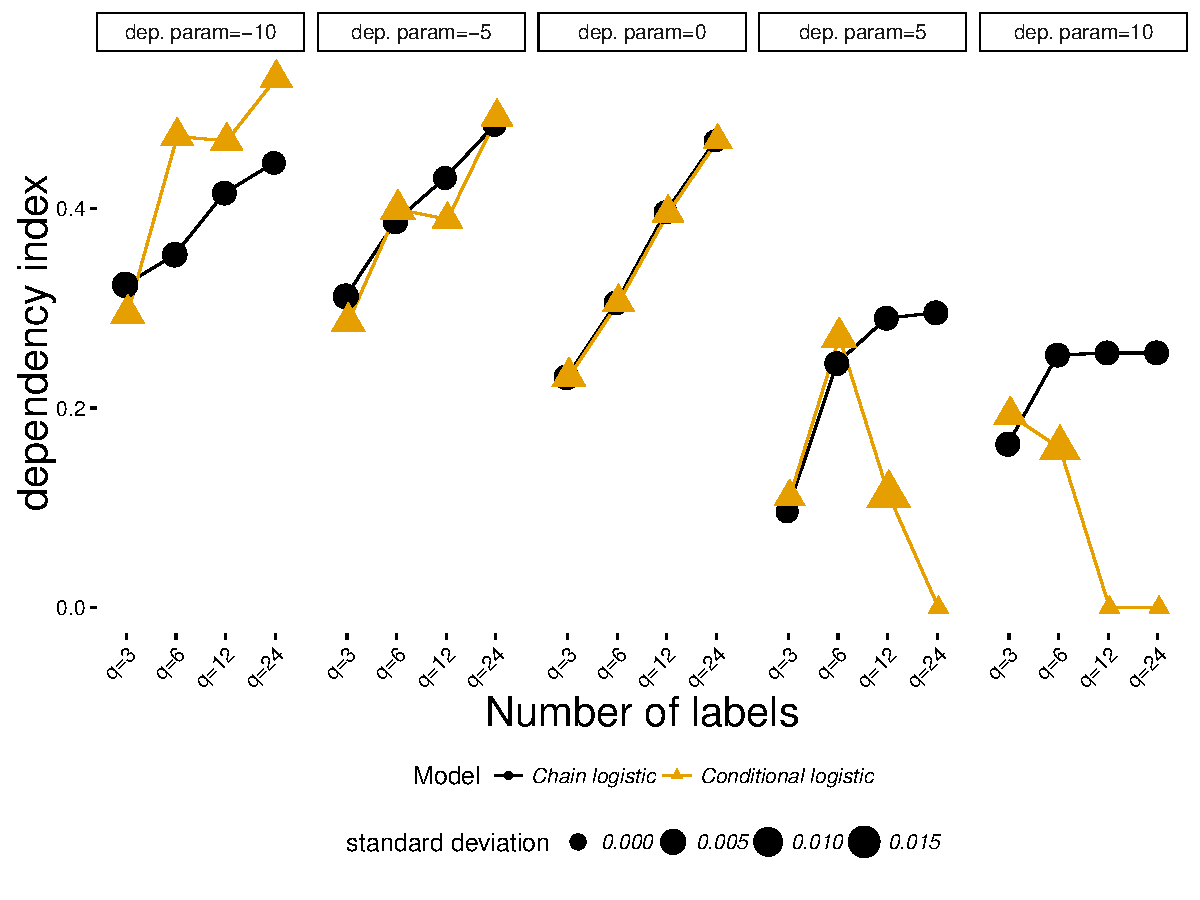
\includegraphics[width=0.49\textwidth]{ud_q.pdf}
				}\\
    \subfigure[Varying $\gamma$, $\theta$ \& $p$]{%
        \label{fig:results:dep:cd:p}
        \includegraphics[width=0.49\textwidth]{cd_p.pdf}
				}%
    \subfigure[Varying $\gamma$, $\theta$ \& $q$]{%
        \label{fig:results:dep:cd:q}
        \includegraphics[width=0.49\textwidth]{cd_q.pdf}
				}%
		\end{center}
    \caption{{\bf This plot needs to be re-drawn from new experiments: remove the probit model; change the values of $p$ and $q$ to the 4 small numbers.} Unconditional and conditional dependence: (a) and (b) unconditional dependence; (c) and (d) conditional dependence.}
    \label{fig:results:dep}
\end{figure}

We can observe from Figure~\ref{fig:results:dep} the followings.

Firstly, {\bf To be elaborated by describing the pattern in unconditional and conditional dependence as the dependence parameters increase.  Also, Can we delete conditional dependence from this paper?  It seems it has no increasing trend, which makes me doubt the statistical test is a good way to represent conditional dependence. First describe observations and then provide explanation as follows.}
We call \emph{dependence parameters} those represented by $\gamma_{ji}$ and $\theta_{ij}$ in (\ref{eq:cc}) and (\ref{JC}), respectively. For the chain of logistic regressions and conditional logistic regressions models, these dependence parameters are interpreted as conditional log-odds ratios. By altering the value of these parameters we affect $P(y_{j} = 1|\mathbf{x},\mathbf{y}_{subset})$. For this reason, we expect an increasing/decreasing trend of unconditional and conditional dependence among the labels as we increase/decrease the value of the dependence parameters. 

Secondly, The unconditional dependency measurements are tampered by label imbalance, when varying $q$. This is why we fail to observe the expected pattern (higher increase in unconditional dependence of conditional logistic regressions model). 

Thirdly, {\bf To be elaborated.} Conditional dependence is less affected: we expected an increase in it as $p$ grows, since we are increasing the set of conditioning variables. We can observe that this happens as the number of predictors increase. On the other hand, we expect a decrease in conditional dependence as the number of labels $q$ grow, because the set of conditioning variables remains unchanged (fixed $p$) but the measured variables increase. 
{\bf Then explanation:}
For fixed values of dependence parameters and $q$, we expect a nonlinear decreasing trend on label density, imbalance, unconditional and conditional dependence as $p$ grows, because other labels will have less and less influence on a certain label as more and more influence is exerted by the increasing number of predictors. The pattern will be nonlinear because the predictors' other characteristics (than the number of predictors) will still exert some impact on data's multi-label attributes.

Finally, {\bf To be elaborated.} Additionally, as the number of labels and the dependence parameters increase, cardinality increases as well. This is, the are more frequent co-occurrences of ones between labels. So, with a fixed conditioning set and similar labels, measurements are likely to be the same (that is why also standard deviation decreases as we increase the number of labels $q$).
{\bf Then explanation:}
	For fixed values of dependence parameters and $p$, we expect a nonlinear increasing trend in the number of ones per instance {\bf as well as per label??} as the number of labels increases. Ideally, we would expect an increasing trend on unconditional and conditional dependence. The dependence parameters are the same for all labels, so it is more likely that the labels will increase their dependence on each other as $q$ grows. However, as the number of ones (or zeros) gets larger, metrics will be affected. Thus, we may see sudden rises or descents in both dependences originated by co-occurrence and imbalance of labels. Nonetheless, we expect the overall trend of the dependences to be upwards as $q$ increases.

{\bf Some intuitive explanation can be done by recycling the text following.}
From our toy example (\ref{TOY}), we learned that as the value of the dependence parameters increases the probability of co-occurring ones increases as well. This leads to think that both unconditional and conditional dependence will behave similarly; i.e., they will increase as the dependence parameters increase. We also saw that label imbalance increases as the value of the dependence parameters grows. This affects unconditional dependency because it relies on correlation. If there are datasets whose labels columns are all ones (or zeros), then there would be no variability and, therefore, no means to measure correlation between those labels (we only need one of the labels to have no variability). The contribution of labels in this situation is not included for the final measurement. The value recorded represents a lower unconditional dependency than what it truly is.


\subsubsection{Label imbalance}

\begin{figure}[H]
    \begin{center}
    \subfigure[Varying $\gamma$, $\theta$ \& $p$]{
        \label{fig:results:imb:p}
        \includegraphics[width=0.49\textwidth]{li_p.pdf}
				}%
    \subfigure[Varying $\gamma$, $\theta$ \& $q$]{
        \label{fig:results:imb:q}
        \includegraphics[width=0.49\textwidth]{li_q2609.pdf}
				}
		\end{center}
    \caption{{\bf This plot needs to be re-drawn from new experiments: remove the probit model; change the values of $p$ and $q$ to the 4 small numbers.}  Label imbalance. We can observe an increasing trend in label imbalance index as we increase the value of the models' dependence parameters, from \texttt{b1} to \texttt{b5} denoting the five values in ascending order of $\gamma$ and $\theta$ in (\ref{eq:param:gamma}) and (\ref{eq:param:theta}), respectively. We can also see that as we increase the number of predictors $p$, the degree of label imbalance decreases; and as we increase the number of labels $q$, the degree of label imbalance increases.}
    \label{fig:results:imb}
\end{figure}

The plots for the label imbalance index, measured from the datasets simulated by the two statistical models, is shown in Figure~\ref{fig:results:imb}, from which we can make four observations.

Firstly, as we increase the value of the dependence parameters, the degree of label imbalance increases. 
{\bf Then add explanation:}
	An increase/decrease in $P(y_{j} = 1|\mathbf{x},\mathbf{y}_{subset})$'s conditional odds ratio will also affect the co-occurrence of ones and zeros in an instance. That is, we expect a larger number of ones/zeros per instance as well as per label. Thus, we expect density {\bf and label imbalance???} to increase as we increase the value of dependence parameters.  


Secondly, when we increase the number of predictors $p$, the degree of label imbalance decreases.

Thirdly, contrary to what happens to $p$, as we increase the number of labels $q$, the degree of label imbalance increases.

Finally, the conditional logistic regressions model renders the higher increase and values in label imbalance than the chain of logistic regressions model, as the magnitude of dependence parameters increase (with everything else fixed).
To build intuition for this, we define a simplified model with one predictor $x$ and three labels $y_{1}$, $y_{2}$ and $y_{3}$ with following parameters (chosen arbitrarily):
%
\begin{equation}\label{TOY}
x = 0.41, \quad \beta_{y_{1}} = \left(\begin{array}{r} 0.97\\-1.14 \end{array} \right), \quad \beta_{y_{2}} = \left(\begin{array}{r} 0.63\\1.89 \end{array} \right), \quad \beta_{y_{3}} = \left(\begin{array}{r} 1.40\\0.26 \end{array} \right).
\end{equation}
{\bf Why here $\beta$ is a vector, not a scalar?  Also, why not let $0< \beta_1 < \beta_2 < \beta_3$ to investigate a pattern between labels?}
%
The marginal distributions of the labels are functions of $x,\beta_{y_{1}},\beta_{y_{2}},\beta_{y_{3}}$ and $\gamma$ or $\theta$, depending on the model. We fix the values of $x$ and $\beta_{y_{i}}$ for $i \in \{1, 2, 3\}$ to depict the patterns of the marginal distributions when we vary their dependence parameters, namely $\gamma$ and $\theta$, in From Figure \ref{fig:results:imb:toy}.  
We can observe that the probability of $y_{i}=1$ is higher and closer to 1 for the conditional logistic regressions model than the chain of logistic regressions model as their dependence parameters, $\gamma$ and $\theta$, increase. This means that we would expect a larger number of ones for each label in the datasets generated by the conditional logistic regressions model, i.e.~larger label imbalance.

\begin{figure}[H]
    \begin{center}
    \subfigure[{\small Chain logistic}]{
        \label{fig:results:imb:toy:cc}
        \includegraphics[width=0.49\textwidth]{li11.pdf}
				}%
    \subfigure[{\small Conditional logistic}]{
        \label{fig:results:imb:toy:cl}
        \includegraphics[width=0.49\textwidth]{li21.pdf}
				}
		\end{center}
    \caption{Marginal probabilities of labels $y_{i}=1$, for $i=1, 2, 3$, of the chain of logistic regressions model and the conditional logistic regressions model.}
    \label{fig:results:imb:toy}
\end{figure}


\subsubsection{Label density}

\begin{figure}[H]
    \begin{center}
    \subfigure[Varying $\gamma$, $\theta$ \& $p$]{
        \label{fig:results:density:p}
        \includegraphics[width=0.49\textwidth]{dn_p2609.pdf}
				}%
    \subfigure[Varying $\gamma$, $\theta$ \& $q$]{
        \label{fig:results:density:q}
        \includegraphics[width=0.49\textwidth]{de_q2609.pdf}
				}
		\end{center}
    \caption{{\bf This plot needs to be re-drawn from new experiments: remove the probit model; change the values of $p$ and $q$ to the 4 small numbers.} Label density (the mean number of ones (active labels) per instance). We observe an increase in this value as the dependence parameters grow.}
    \label{fig:results:density}
\end{figure}

From Figure~\ref{fig:results:density}, we can make three observations.

Firstly, there is an increase in the value of label density as the dependence parameters grow. {\bf To be elaborated a bit.}

Secondly, the conditional logistic regressions model has, on average, a higher increase in cardinality as its dependence parameters increase.  {\bf To be elaborated a bit.}

Thirdly, there seems no clear pattern with the increasing $p$ or $q$.  {\bf To be elaborated a bit and delete/revise the text following.}  Also, we can see two different patterns. When we increase the number of predictors $p$, the density seems to converge to 0.5. On the other hand, as we increase the number of labels $q$ the cardinality increases as well. Although, the increase is not monotonic. It seems that it first reaches a minimum value and then it grows as $q$ grows. These two patterns suggest that the dependence parameters have more influence in cardinality than the number of predictors $p$.


\section{Conclusion}
\label{CONCL} %Limitations of the study, scope. Focus on statistical models. No generalisation. Give possible reasons (with arguments) about the results of experiments. Are there new unexpected results/patterns?

In this paper we conducted several experiments aiming to discover the patterns elicited in multi-label attributes when data were generated by two statistical models, namely chain of logistic regressions and conditional logistic regressions. We commented about how to measure synthetic data's multi-label attributes. In addition, we proposed a simple way to visualise and measure label imbalance.

The conditional logistic regressions model renders the highest increase of the attributes measured when its dependence parameter $\theta$ is increased,  for fixed number of predictors and labels. Using the experiments' simple dependency setting, this model is useful when high degrees of unconditional dependence, cardinality and label imbalance are required. If the user wants high unconditional dependence, it is important to monitor label imbalance to avoid unwanted issues related with it. On the other hand, if for some reason the user needs high label imbalance then this model is the most useful choice among the two models.

The chain of logistic regressions model increases less than the conditional logistic regressions model as its dependence parameter $\gamma$ grows. This makes the model useful for simulating data with dependent labels and moderate label imbalance and cardinality. It is important to remind the reader that, for multi-label learning, the order in which labels are generated matters for the chain of logistic regressions model. Thus, it is important to keep record of label ordering and/or treat it as an extra parameter.


\section*{Acknowledgements}
M. Valencia Garza gratefully acknowledges a scholarship from Consejo Nacional de Ciencia y Tecnologia (CONACyT).

\section*{References}

\bibliographystyle{elsarticle-num-names}
\bibliography{MLC-simulation}

\end{document}

\endinput

